%&LaTeX
\documentclass[11pt,a4paper]{article}
\usepackage[frenchb,english]{babel}
\usepackage[applemac]{inputenc}
\usepackage[OT1]{fontenc}
\usepackage[]{graphicx}
\usepackage{amsmath}
\usepackage{amsfonts}
\usepackage{amsthm}
\usepackage{amssymb}
\usepackage{tikz}
\graphicspath{ {./figures/} }
%\input{8bitdefs}

% marges
\topmargin 10pt
\headsep 10pt
\headheight 10pt
\marginparwidth 30pt
\oddsidemargin 40pt
\evensidemargin 40pt
\footskip 30pt
\textheight 670pt
\textwidth 420pt

\def\imp{\Rightarrow}
\def\gcro{\mbox{[\hspace{-.15em}[}}% intervalles d'entiers 
\def\dcro{\mbox{]\hspace{-.15em}]}}

\newcommand{\be} {\begin{enumerate}}
\newcommand{\ee} {\end{enumerate}}
\newcommand{\deb}{\begin{eqnarray*}}
\newcommand{\fin}{\end{eqnarray*}}
\newcommand{\ssi} {si et seulement si }
\newcommand{\D}{\mathrm{d}}
\newcommand{\Q}{\mathbb{Q}}
\newcommand{\Z}{\mathbb{Z}}
\newcommand{\N}{\mathbb{N}}
\newcommand{\R}{\mathbb{R}}
\newcommand{\C}{\mathbb{C}}
\newcommand{\F}{\mathbb{F}}
\newcommand{\U}{\mathbb{U}}
\newcommand{\re}{\,\mathrm{Re}\,}
\newcommand{\im}{\,\mathrm{Im}\,}
\newcommand{\ord}{\mathrm{ord}}
\newcommand{\Gal}{\mathrm{Gal}}
\newcommand{\legendre}[2]{\genfrac{(}{)}{}{}{#1}{#2}}


\title{Solutions to David A.Cox  "Galois Theory''}

\refstepcounter{section} \refstepcounter{section}
\refstepcounter{section} \refstepcounter{section}
\refstepcounter{section}\refstepcounter{section}\refstepcounter{section}\refstepcounter{section}
\refstepcounter{section}\refstepcounter{section}\refstepcounter{section}\refstepcounter{section}\refstepcounter{section}


\begin{document}



\section{Chapter 15 : THE LEMNISCATE}

\subsection{DIVISION POINTS AND ARC LENGTH}

\paragraph{Ex. 15.1.1}{\it Prove that the numbers described in Abel's theorem at the beginning of the chapter are precisely those in Theorem 10.2.1, provided we replace ``product of several numbers'' with ``product of distinct numbers'' in Abel's statement of the theorem.
}
\begin{proof}
The numbers described in Theorem 10.2.1 are the integers $n = 2^s p_1\cdots p_r$, where $p_1,\ldots,p_r$ are distinct Fermat primes, of the form $p_k = 2^{n_k} + 1$. Thus these numbers are the product of {\it distinct} numbers of the form $2^m$, or $2^{m}+1$, where $2^{m} + 1$ is prime, as described in the Theorem of Abel.
\end{proof}

\paragraph{Ex. 15.1.2}{\it Show that in polar coordinates, the equation of the lemniscate is $r^2 = \cos(2\theta)$.
}
\begin{proof}
By definition, a point $M = (x,y) \in \R^2$ is a point of the lemniscate $L$ if and only if
$$(x^2 + y^2)^2 = x^2 - y^2.$$ 
If $(r,\theta)$ are polar coordinates of $M = M(r,\theta)$, then $x = r \cos\theta, y = r \sin\theta$, thus, using $\cos^2 \theta + \sin^2 \theta = 1$, and $\cos(2\theta) = \cos^2 \theta) - \sin^2 \theta$, we obtain
\begin{align*}
M(r,\theta) \in L & \iff (r^2 \cos^2\theta + r^2 \sin^2\theta)^2 = r^2 \cos^2\theta - r^2 \sin^2\theta\\
&\iff r^4 = r^2 \cos(2\theta)\\
&\iff r^2 = \cos(2\theta).
\end{align*}
The equation of the lemniscate is $r^2 = \cos(2\theta)$.
\end{proof}


\paragraph{Ex. 15.1.3}{\it Prove that the two improper integrals $\int_0^1 (1-t^4)^{-1/2} \mathrm{d}t$ and $\int_{-1}^0 (1-t^4)^{-1/2} \mathrm{d}t$ converge.
}
\begin{proof}
 The map $t \mapsto (1-t^4)^{-1/2}$ is continuous on $[0,1[$, thus $t \mapsto(1-t^4)^{-1/2} \mathrm{d}t$ is summable on $[1,x]$ for all $x \in [0,1]$.  

Since $1-t^4 = (1-t)(1+t+t^2+t^3)$, $(1-t^4)^{-1/2} \sim [4(1-t)]^{-1/2}$ in the neighborhood of $1$. The Riemann Criterium shows that $\int_0^1 (1-t)^{-\alpha} \mathrm{d}t$ converges if  $\alpha  < 1$, and here $\alpha = 1/2$. Since $(1-t^4)^{-1/2} >0$, this is sufficient to prove that $\int_0^1 (1-t^4)^{-1/2} \mathrm{d}t$ converges.

Since $t \mapsto (1-t^4)^{-1/2}$ is even, the same is true in the neighborhood of $-1$, thus $\int_{-1}^0 (1-t^4)^{-1/2} \mathrm{d}t$ converges.
\end{proof}

\paragraph{Ex. 15.1.4}{\it  Prove the arc length formula stated in (15.6)}
\begin{proof}
 Here the equation of th ellipse $E$ is
 $$x^2 + \frac{y^2}{b^2} = 1,$$
 with eccentricity $k = \sqrt{1- b^2}$.

We compute the arc length $l$ of (E) between $x = u, y=v\ (-1<u<v<1)$ on the upper part of the curve. Then
$$l =  \int_u^v \sqrt{1+\left( \frac{\D y}{\D x}\right)^2}\  \D x,$$
where $y = f(x) = b \sqrt{1-x^2}.$ Then $f'(x) =  \frac{\D y}{\D x }= -\frac{2x}{\sqrt{1-x^2}}$, thus
\begin{align*}
l &=  \int_u^v \sqrt{1+\left(\frac{bx}{\sqrt{1-x^2}}\right)^2}\  \D x\\
&=\int_u^v \sqrt{\frac{1 - x^2 + b^2 x^2}{1-x^2}}\  \D x\\
&=\int_u^v \sqrt{\frac{1 - k^2 x^2}{1-x^2}}\  \D x\\
\end{align*}
We have proved
$$l =  \int_u^v \sqrt{1+\left( \frac{\D y}{\D x}\right)^2}\  \D x = \int_u^v \sqrt{\frac{1 - k^2 x^2}{1-x^2}}\  \D x = \int_u^v \frac{\sqrt{(1-x^2)(1 - k^2 x^2)}}{1-x^2}\  \D x.$$
The arc length of the ellipse is given by an elliptic integral.
\end{proof}

\paragraph{Ex. 15.1.5}{\it  Shows that (15.7) reduces to $(x^2+y^2)^2 = x^2 -y^2$ when $a=b = 1/\sqrt{2}$.
}
\begin{proof}
 If we take $a=b=1/\sqrt{2}$ in the formula of the ovals of Cassini
 $$((x-a)^2 + y^2)((x+a)^2 + y^2) = b^4,$$
 we obtain
 \begin{align*}
 \frac{1}{4} &= \left[ \left(x - \frac{1}{\sqrt{2}} \right)^2 + y^2\right ] \left[ \left(x + \frac{1}{\sqrt{2}} \right)^2 + y^2\right ]  \\
 &=\left( x^2+y^2 +\frac{1}{2}  - \sqrt{2}\, x \right)\left( x^2+y^2 +\frac{1}{2}  + \sqrt{2}\, x \right)\\
 &=\left((x^2 + y^2 + \frac{1}{2}\right)^2 - 2 x^2\\
 &=(x^2+y^2)^2  + (x^2+y^2) - 2 x^2\\
 &= (x^2+y^2)^2 + y^2 -x^2 + \frac{1}{4}.
 \end{align*}
 Therefore, for $a=b =1/\sqrt{2}$, the equation $((x-a)^2 + y^2)((x+a)^2 + y^2) = b^4$ reduces to
 $$(x^2 + y^2)^2 = x^2 - y^2,$$
 which is the equation of the Lemniscate.
\end{proof}
\paragraph{Ex. 15.1.6}{\it Let $n>0$ be an odd integer, and assume that the $n$-division points of the lemniscate can be constructed with straightedge and compass. prove that the same is true for the $2n$-division points. Your proof should include a picture.
}

\begin{proof} Let $M_0=0, \ldots,M_{n-1}$ the $n$-divisions points
If $n$ is odd, the middle segment $(M_{(n-1)/2}, M_{(n+1)/2})$ straddles the origin, The symmetry of the figure shows that the arc length between $O$ and $M_{(n-1)/2}$ is the same as the arc length between $O$ and $M_{(n-1)/2}$, so is half of the arc length $M_k M_{k+1}$. Therefore we can complete $M_0, M_1, \ldots,M_{n-1}$ by the symmetric points $M'_0 = O,\ldots,M'_{n-1}$ relative to the $x$-axis to obtain the $2n$-division points (the point $O$ is counted twice).

Figure for $n=5$ : the $10$-division points are $0,M'_2,M_1,M'_1,M_2,0,M_3,M'_3,M_4,M'_3$.
\begin{figure}[htbp]
\begin{center}
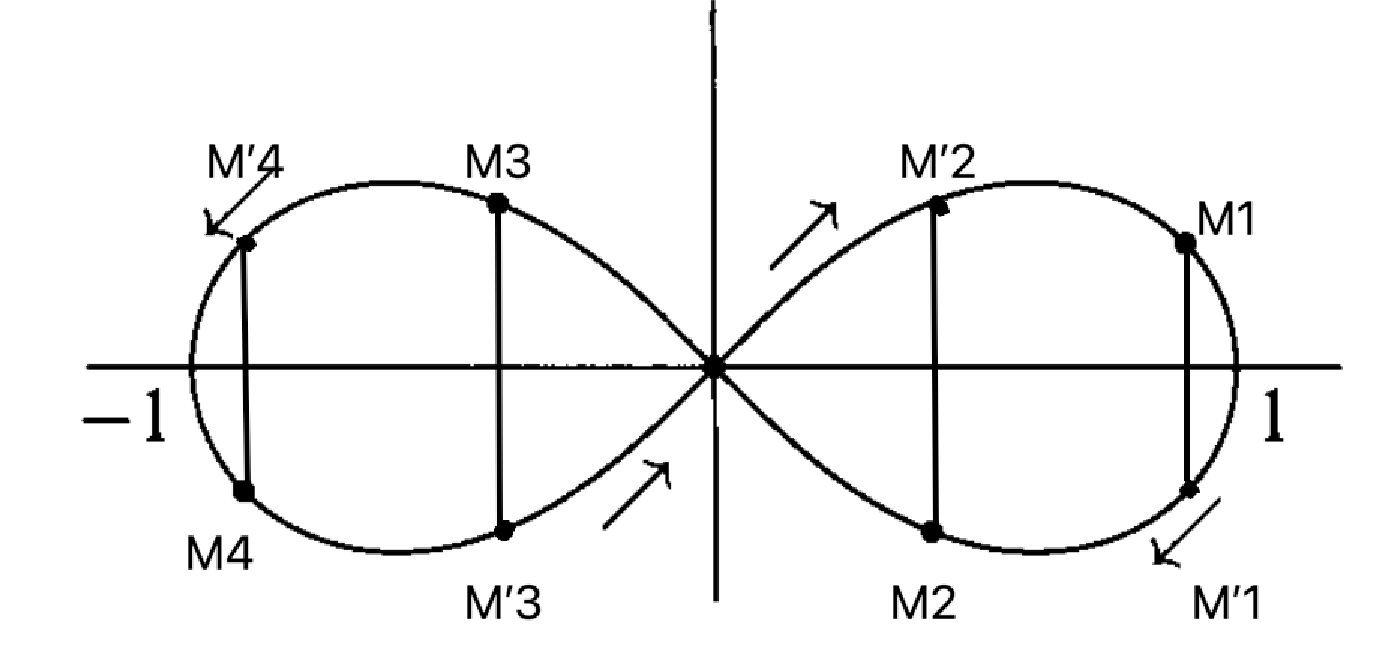
\includegraphics [width=8cm,height=4cm] {lemniscate.png}
\end{center}
\end{figure}
\end{proof}

\paragraph{Ex. 15.1.7}{\it Recall that in Greek geometry, the ellipse is defined to be the locus of all points whose {\bf sum} of distances to two given points is constant. Suppose instead we consider the locus of all points whose {\bf product} of distances to two given points is constant. Show that this leads to (15.7) when the given points are $(a,0),(-a,0)$ and the constant is $b^4$(*).
}

(*) Read $b^2$.

\begin{proof}
Let $\Gamma$ the locus of all points whose product of distances to two points $(a,0),(-a,0)$ is the constant $b^2$. Then
\begin{align*}
M(x,y) \in \Gamma & \iff \sqrt{(x-a)^2 + y^2}   \sqrt{(x+a)^2 + y^2}  = b^2\\
&\iff ((x-a)^2 + y^2)((x-a)^2 + y^2) = b^4.
\end{align*}
We obtain the formula of the ovals of Cassini.
\end{proof}


\subsection{THE LEMNISCATIC FUNCTION}
\paragraph{Ex. 15.2.1}{\it Give a careful proof of (15.9) using the hints given in the text.
}

\begin{proof}
By section 15.2, we know that $\varphi$ is $2\varpi$ periodic,
$$\varphi(s + 2\varpi) = \varphi(s),\qquad (s \in \R).$$
Moreover, for $-1 \leq r \leq 1$, and $\frac{-\varpi}{2} \leq s \leq \frac{\varpi}{2}$,
$$r = \varphi(s) \iff s = \int_0^r \frac{1}{\sqrt{1-t^4}} \D t.$$

Write $r' = \varphi(-s)\in [-1,1]$. Then for every $s \in [-\frac{\varpi}{2} ,\frac{\varpi}{2} ]$,
\begin{align*}
r' = \varphi(-s) & \iff -s = \int_0^{r'} \frac{1}{\sqrt{1-t^4}} \D t\\
&\iff -s = -\int _0^{-r'} \frac{1}{\sqrt{1-\tau^4}} \D \tau\qquad (\tau = -t)\\
&\iff s = \int _0^{-r'} \frac{1}{\sqrt{1-\tau^4}} \D \tau\\
&\iff -r' = \varphi(s)
\end{align*}
This proves that
\begin{align}
\varphi(-s) = - \varphi(s) \qquad \left (-\frac{\varpi}{2} \leq s \leq \frac{\varpi}{2} \right).
\end{align}

Write $M(s)$ the point on the lemniscate with signed arc length $s$. Consider $M' = M(s')$ the symmetric point of $M(s)$ about the origin. Since the lemniscate is symmetric about the origin, 
Consider first the case where $0 \leq s \leq \varpi$, then the signed arc length is the positive arc length. Let $M(s)$ the point on the lemniscate with arc length $s$. Then the symmetric point $M(s')$ about the $x$-axis is such that $r' = OM(s') = OM(s) = r$, thus, by definition of $\varphi$, $\varphi(s) = \varphi(s')$. The total arc length from $O = M(0)$ to $O = M(\varpi)$ in the first loop is $\varpi$, and the symmetry of the lemniscate about the $x$-axis implies that the arc length $\varpi - s$ between $M(s)$ and $O = M(\varpi)$ is equal to the arc length $s'$ between $O = M(0)$ and $M(s')$, thus
$s' = \varpi - s$. This proves
\begin{align}
\varphi(\varpi -s) = \varphi(s)\qquad (0 \leq s \leq \varpi).
\end{align} 

Now, if $\frac{\varpi}{2} \leq s \leq \varpi$, then $0\leq \varpi-s \leq \frac{\varpi}{2}$, thus, using (1), (2), (3)
$$
\left\{
\begin{array}{ll}
\varphi(s) &= \varphi(\varpi - s) = -\varphi(s- \varpi) = -\varphi(s + \varpi),\\
\varphi(-s) &= \varphi(\varpi- (-s)) =\varphi(s + \varpi).
\end{array}
\right.
$$
Therefore $\varphi(-s) = - \varphi(s)$ if $\frac{\varpi}{2} \leq s \leq \varpi$. Now, if we suppose $-\varpi \leq s \leq -\frac{\varpi}{2}$, then $\frac{\varpi}{2} \leq -s \leq \varpi$, so we can apply the last equality to $-s$: $\varphi(s) = \varphi(-(-s))= - \varphi(-s)$. This proves
\begin{align}
\varphi(-s) = \varphi(s) \qquad (-\varpi \leq s \leq \varpi).
\end{align}
Using the periodicity, if $s \in \R$, the is some $n \in \Z$ and $s' \in [-\varpi,\varpi[$ such that $s = 2n\varpi + s'$. Then 
$$\varphi(-s) = \varphi(-s - 2n\varpi) = \varphi(-s') = - \varphi(s') = -\varphi(s-2n\varphi) = - \varphi(s).$$
 We have proved
$$\varphi(-s) = \varphi(s) \qquad (s \in \R).$$
We can now complete (2) to $-\varpi \leq s \leq 0$. Then $0 \leq -s \leq \varpi$, and by (2) applied to $-s$, $\varphi(s + \varpi) = \varphi(-s) = -\varphi(s)$, thus
$$\varphi(\varpi -s) =  - \varphi(s - \varpi) = - \varphi(s+ \varpi) = \varphi(s)$$.

We have proved, for all $s \in \R$,
\begin{align*}
&\varphi(-s) = -\varphi(s)\\
&\varphi(\varpi - s) = \varphi(s).
\end{align*}
\end{proof}

\paragraph{Ex. 15.2.2}{\it Supply the details needed to complete the proof of Proposition 15.2.1.
}

\begin{proof}
The proof of Proposition 15.2.1 shows that
$$\varphi'(s)  = \sqrt{1 - \varphi^4(s)},\qquad 0 \leq s \leq \frac{\varpi}{2}.$$
By Exercise 3, part (a) and (b), $\varphi'$ is even and has period $2 \varpi$. 
Moreover, taking the derivative of $s \mapsto \varphi(\pi - s) = \varphi(s)$ on $\R$, we obtain $-\varphi'(\varpi - s) = \varphi'(s)$, thus
$$\varphi'(\varpi - s) = - \varphi'(s), \qquad s \in \R.$$

Therefore, if $-\frac{\varpi}{2} \leq s \leq 0$, then
$$\varphi'(s) = - \varphi'(-s) =  -\sqrt{1 - \varphi^4(-s)} = - \sqrt{1 - \varphi^4(s)}.$$
Now, if $\frac{\varpi}{2} \leq s \leq \varpi$, then $0 \leq \varpi -s \leq \frac{\varpi}{2}$, thus 
$$\varphi'(s) = -\varphi'(\varpi - s) = -\sqrt{1 - \varphi^4(\varpi - s)} = - \sqrt{1 - \varphi^4(s)}.$$
If $-\varpi \leq s \leq -\frac{\varpi}{2}$, then $\frac{\varpi}{2} \leq -s  \leq \varpi$. Using the above equality, we obtain
$$\varphi'(s) = - \varphi(-s) = -  \sqrt{1 - \varphi^4(-s)} = - \sqrt{1 - \varphi^4(s)}.$$
We have proved
$$\varphi'^2(s) = 1 - \varphi^4(s), \qquad -\varpi \leq s \leq \varpi. $$
Now if $s$ is any real number, there is some $n\in \Z$ and $s' \in [-\varpi, \varpi[$ such that $s = 2n \varpi + s'$. Since $2\varpi$ is a period of $\varphi$ and $\varphi'$,
$$\varphi'^2(s) = \varphi'^2(s') = 1 -\varphi^4(s') = 1 - \varphi^4(s).$$
This complete the proof of Proposition 15.2.1.
\end{proof}

\end{document}
